\documentclass[a4paper]{article}

%% Language and font encodings
\usepackage[brazil]{babel}
\usepackage[utf8x]{inputenc}
\usepackage[T1]{fontenc}

%% Sets page size and margins
\usepackage[a4paper,top=3cm,bottom=2cm,left=3cm,right=3cm,marginparwidth=1.75cm]{geometry}

%% Useful packages
\usepackage{amsmath}
\usepackage{graphicx}
\usepackage[colorinlistoftodos]{todonotes}
\usepackage[colorlinks=true, allcolors=blue]{hyperref}
\usepackage{multicol,multirow}

\title{IF690 - História e Futuro da Computação}
\author{Eidson Sá}
\date{}
\begin{document}
\maketitle

\section{Introdução}
	A matéria de História e Futuro da Computação \cite{HC:2007:CFF} tem como objetivo falar sobre a história da computação a partir de eventos importantes de forma a entender como estes ajudaram a moldá-la. Além disso, a matéria trata de temas como \textit{Deep Web}, \textit{Hackers}, Internet das Coisas, \textit{Big Data}, Cidades inteligentes e \textit{Cybercoins}. Analisando o passado, também consegue recolher estatísticas e projetar o que deve ser tendência no futuro no ramo da computação. A cadeira se insere em quase todas as áreas da computação, por tratar de mostrá-las aos alunos.

\begin{figure}[h]
\centering

\includegraphics[width=0.3\textwidth]{ejas1.png}
\caption{\label{fig:bit}Bitcoin, uma das mais importantes Cybercoins, tópico estudado na disciplina. (CC-0)}
\end{figure}

\begin{figure}[h]
\centering
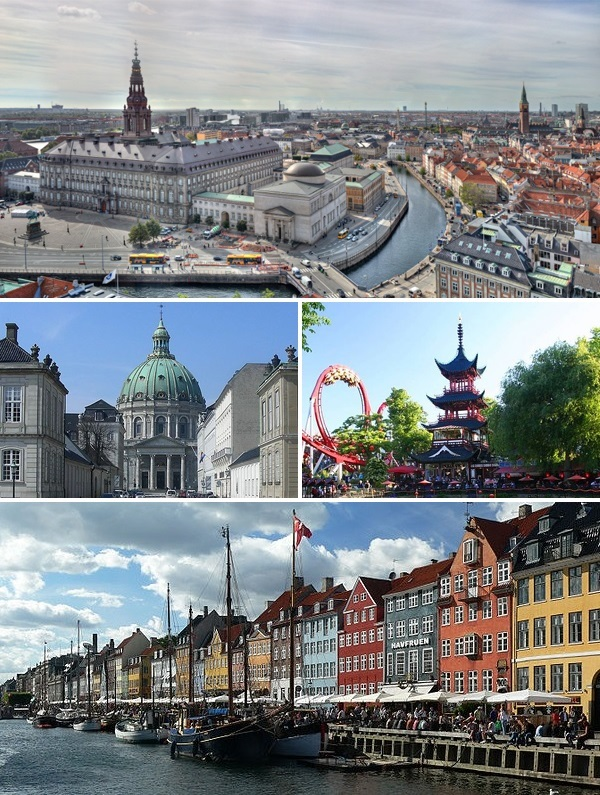
\includegraphics[width=0.4\textwidth]{ejas2.jpg}
\caption{\label{fig:cop} Copenhague, uma das mais famosas cidades inteligentes, tópico estudado na disciplina. (CC BY-SA 3.0)}
\end{figure}

\section{Relevância}
	A disciplina de História e Futuro da Computação tem grande importância para o currículo de Ciências da Computação, pois faz com que o aluno entenda o passado e a evolução da Computação, sendo capaz o mesmo de entender o porquê de certos fatos terem ocorrido e usá-los como base para o futuro de sua profissão e para sua entrada no mercado de trabalho. Além disso, trata de temas distintos que podem ser úteis para mostrar ao aluno modos diferentes de trabalho relacionados à computação. Existem algumas vantagens e desvantagens de se ter essa matéria: 

\begin{itemize}
\item Prós
\begin{itemize}
\item Faz o aluno se interessar por temas diversos relacionados à computação, ao mostrar a relação entre eles, sua história e como são utilizados;
\item Leva o aluno a pensar na sua carreira, em âmbitos sociais, ao relacionar o passado da computação com o futuro.
\end{itemize}
\item Contras
\begin{itemize}
\item Por ser algo diferente da maioria e se distanciar da Matemática e da Informática Prática, pode se tornar um empecilho para o aluno;
\item Por mais que mostre diversos tópicos, acaba sendo repetitiva e falando de determinados assuntos que já são conhecidos pelos alunos.
\\
\\
\end{itemize}
\end{itemize}

\section{Relação com outras disciplinas}

\begin{table}[h]
\centering
\begin{tabular}{|l|l|}
\hline
Disciplinas                        & Relação com História e Futuro da Computação                                                                                                                      \\ \hline
IF679 - Informática e Sociedade \cite{IF679}   & \begin{tabular}[c]{@{}l@{}}Também fala da computação de maneira mais humana, tratando,\\  principalmente, da relação entre Informática e ser humano\end{tabular} \\ \hline
IF668 - Introdução à Computação  \cite{IF668}  & \begin{tabular}[c]{@{}l@{}}Também tem o trabalho de mostrar diversos temas relacionados \\ à Computação aos alunos e falar sobre seu surgimento\end{tabular}    \\ \hline
IF691 - Trabalho de Graduação (TG) & \begin{tabular}[c]{@{}l@{}}Também tem como método de avaliação um texto redigido, uma\\  tese, ao invés das tradicionais provas.\end{tabular}                                                      \\ \hline
\end{tabular}
\end{table}
\bibliographystyle{ieeetr}
\bibliography{ejas}

\end{document}